%%!TEX encoding = UTF-8 Unicode

\documentclass{article}
\usepackage[utf8]{inputenc}
\usepackage[T1]{fontenc} % Use 8-bit encoding that has 256 glyphs

\usepackage{tikz}
\tikzset{node distance=2cm, auto}

\begin{document}

Assumindo que existe uma função $f$ tal que

\begin{tikzpicture}
  \node (B) {$A$};
  \node (C) [right of=B]{$B$};
  
  \draw[->] (B) to node {$f$} (C);

  %\draw[->, dashed] (C) to node [swap] {$\langle f_i \rangle_{i \in I}$} (P);
  %\draw[->] (P) to node [swap] {$\pi_i$} (Ai);
\end{tikzpicture}

e que a relação curry é a seguinte:


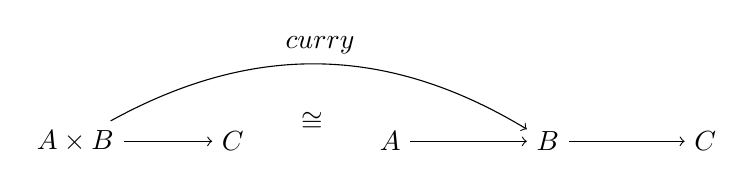
\begin{tikzpicture}
  \node (B) {$A \times B$};
  \node (C)[right of= B] {$C$};
  \node(D)[right of= C] {$A$};
  \node (E)[right of= D] {$B$};
  \node (F) [right of= E]{$C$};


  %\draw[->, dashed] (C) to node [swap] {$\langle f_i \rangle_{i \in I}$} (P);
  %\draw[->] (P) to node [swap] {$\pi_i$} (Ai);
  \draw[->](B) to node [distance =1cm] {} (C);
  \draw[white] (C) edge node[black, distance=1cm] {$\cong$} (D);
  
  \draw[->](D) to node {} (E);
    \draw[->](E) to node {} (F);
 \draw [->](B) edge[bend left] node [above]{$curry$} (E);
  
\end{tikzpicture}



então


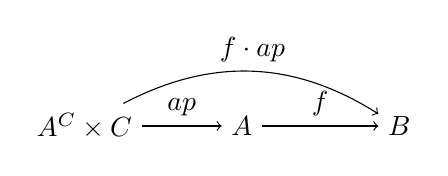
\begin{tikzpicture}
  \node (A) {$A^C \times C$};
  \node (B) [right of=A]{$A$};
  \node (C) [right of=B]{$B$};
  
%  \draw[->] (A) to node {$f \cdot ap$} (C);
  \draw[->] (A) to node {$ap$} (B);
 \draw[->] (B) to  node {$f$} (C);
 \draw [->](A) edge[bend left] node [above]{$f \cdot ap$} (C);
  %\draw[->, dashed] (C) to node [swap] {$\langle f_i \rangle_{i \in I}$} (P);
  %\draw[->] (P) to node [swap] {$\pi_i$} (Ai);
\end{tikzpicture}

curried

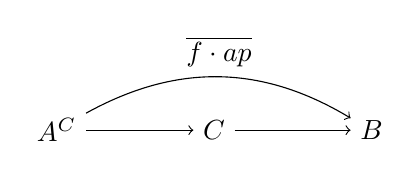
\begin{tikzpicture}
  \node (A) {$A^C$};
  \node (D) [right of=A]{$C$};
  \node (C) [right of=D]{$B$};
  
 \draw[->] (A) to node {$$} (D);
 \draw[->] (D) to node {$$} (C);
  \draw [->](A) edge [bend left] node {$\overline{f \cdot ap}$} (C);

  %\draw[->, dashed] (C) to node [swap] {$\langle f_i \rangle_{i \in I}$} (P);
  %\draw[->] (P) to node [swap] {$\pi_i$} (Ai);
\end{tikzpicture}

simplificando

\begin{tikzpicture}
  \node (A) {$A^C$};
  \node (B) [right of=D]{$B^C$};
  

  \draw [->](A) edge node {$\overline{f \cdot ap}$} (B);

  %\draw[->, dashed] (C) to node [swap] {$\langle f_i \rangle_{i \in I}$} (P);
  %\draw[->] (P) to node [swap] {$\pi_i$} (Ai);
\end{tikzpicture}



\end{document}